\documentclass[a4paper]{article}\usepackage{graphicx, color}
%% maxwidth is the original width if it is less than linewidth
%% otherwise use linewidth (to make sure the graphics do not exceed the margin)
\makeatletter
\def\maxwidth{ %
  \ifdim\Gin@nat@width>\linewidth
    \linewidth
  \else
    \Gin@nat@width
  \fi
}
\makeatother

\definecolor{fgcolor}{rgb}{0.2, 0.2, 0.2}
\newcommand{\hlnumber}[1]{\textcolor[rgb]{0,0,0}{#1}}%
\newcommand{\hlfunctioncall}[1]{\textcolor[rgb]{0.501960784313725,0,0.329411764705882}{\textbf{#1}}}%
\newcommand{\hlstring}[1]{\textcolor[rgb]{0.6,0.6,1}{#1}}%
\newcommand{\hlkeyword}[1]{\textcolor[rgb]{0,0,0}{\textbf{#1}}}%
\newcommand{\hlargument}[1]{\textcolor[rgb]{0.690196078431373,0.250980392156863,0.0196078431372549}{#1}}%
\newcommand{\hlcomment}[1]{\textcolor[rgb]{0.180392156862745,0.6,0.341176470588235}{#1}}%
\newcommand{\hlroxygencomment}[1]{\textcolor[rgb]{0.43921568627451,0.47843137254902,0.701960784313725}{#1}}%
\newcommand{\hlformalargs}[1]{\textcolor[rgb]{0.690196078431373,0.250980392156863,0.0196078431372549}{#1}}%
\newcommand{\hleqformalargs}[1]{\textcolor[rgb]{0.690196078431373,0.250980392156863,0.0196078431372549}{#1}}%
\newcommand{\hlassignement}[1]{\textcolor[rgb]{0,0,0}{\textbf{#1}}}%
\newcommand{\hlpackage}[1]{\textcolor[rgb]{0.588235294117647,0.709803921568627,0.145098039215686}{#1}}%
\newcommand{\hlslot}[1]{\textit{#1}}%
\newcommand{\hlsymbol}[1]{\textcolor[rgb]{0,0,0}{#1}}%
\newcommand{\hlprompt}[1]{\textcolor[rgb]{0.2,0.2,0.2}{#1}}%

\usepackage{framed}
\makeatletter
\newenvironment{kframe}{%
 \def\at@end@of@kframe{}%
 \ifinner\ifhmode%
  \def\at@end@of@kframe{\end{minipage}}%
  \begin{minipage}{\columnwidth}%
 \fi\fi%
 \def\FrameCommand##1{\hskip\@totalleftmargin \hskip-\fboxsep
 \colorbox{shadecolor}{##1}\hskip-\fboxsep
     % There is no \\@totalrightmargin, so:
     \hskip-\linewidth \hskip-\@totalleftmargin \hskip\columnwidth}%
 \MakeFramed {\advance\hsize-\width
   \@totalleftmargin\z@ \linewidth\hsize
   \@setminipage}}%
 {\par\unskip\endMakeFramed%
 \at@end@of@kframe}
\makeatother

\definecolor{shadecolor}{rgb}{.97, .97, .97}
\definecolor{messagecolor}{rgb}{0, 0, 0}
\definecolor{warningcolor}{rgb}{1, 0, 1}
\definecolor{errorcolor}{rgb}{1, 0, 0}
\newenvironment{knitrout}{}{} % an empty environment to be redefined in TeX

\usepackage{alltt}
\usepackage[margin=2cm]{geometry}
\usepackage{graphicx, subfig}


\usepackage[british]{babel}
\usepackage{enumerate}
\IfFileExists{upquote.sty}{\usepackage{upquote}}{}
\begin{document}
\title{STAT 522 || Assignment 3}
%\subtitle{Homework 2}
\author{Subasish Das (sxd1684)}
\maketitle

\section{ Exercise 4.1}

(a)

\begin{knitrout}
\definecolor{shadecolor}{rgb}{0.969, 0.969, 0.969}\color{fgcolor}\begin{kframe}
\begin{alltt}

df_tot = 29
df_err = 20
df_treat = 4
df_block = df_tot - df_treat - df_err
df_block
\end{alltt}
\begin{verbatim}
## [1] 5
\end{verbatim}
\begin{alltt}
m <- \hlfunctioncall{rbind}(df_treat, df_block, df_err, df_tot)
m
\end{alltt}
\begin{verbatim}
##          [,1]
## df_treat    4
## df_block    5
## df_err     20
## df_tot     29
\end{verbatim}
\begin{alltt}

ss_tot = 1503.71
ss_err = 169.33
ss_treat = 1010.56
ss_block = ss_tot - ss_treat - ss_err
ss_block
\end{alltt}
\begin{verbatim}
## [1] 323.8
\end{verbatim}
\begin{alltt}
n <- \hlfunctioncall{rbind}(ss_treat, ss_block, ss_err, ss_tot)
n
\end{alltt}
\begin{verbatim}
##            [,1]
## ss_treat 1010.6
## ss_block  323.8
## ss_err    169.3
## ss_tot   1503.7
\end{verbatim}
\begin{alltt}

ms_treat = ss_treat/df_treat
ms_err = ss_err/df_err
ms_treat
\end{alltt}
\begin{verbatim}
## [1] 252.6
\end{verbatim}
\begin{alltt}
ms_err
\end{alltt}
\begin{verbatim}
## [1] 8.466
\end{verbatim}
\begin{alltt}

ms_block = 64.765

n1 <- \hlfunctioncall{rbind}(ms_treat, ms_block, ms_err)
n1
\end{alltt}
\begin{verbatim}
##             [,1]
## ms_treat 252.640
## ms_block  64.765
## ms_err     8.466
\end{verbatim}
\begin{alltt}

F_treat = 29.84
F_block = ms_block/ms_err
F_block
\end{alltt}
\begin{verbatim}
## [1] 7.65
\end{verbatim}
\begin{alltt}

p_treat = 1 - \hlfunctioncall{pf}(F_treat, df_treat, df_err)
p_treat
\end{alltt}
\begin{verbatim}
## [1] 3.545e-08
\end{verbatim}
\begin{alltt}

p_block = 1 - \hlfunctioncall{pf}(F_block, df_block, df_err)
p_block
\end{alltt}
\begin{verbatim}
## [1] 0.0003689
\end{verbatim}
\end{kframe}
\end{knitrout}


\vspace{3 mm}
\raggedright{The ANOVA Table:}\\
\vspace{2 mm}
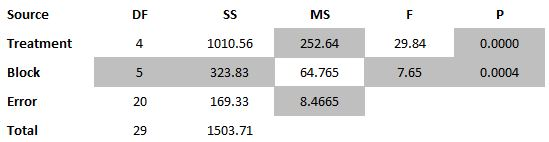
\includegraphics[width=140mm]{fig1.jpg}

\vspace{2 mm}


\raggedright{(b)}
\vspace{2 mm}
Six blocks are used in this experiment.\\
\vspace{2 mm}

(c)
Based on the p-value, we can make decision on the null hypothesis. As for both treatment and block, the p-values are much smaller, we can reject the null hypothesis. \\

\section{ Exercise 4.3}

\begin{knitrout}
\definecolor{shadecolor}{rgb}{0.969, 0.969, 0.969}\color{fgcolor}\begin{kframe}
\begin{alltt}
\hlcomment{## RANDOMIZED BLOCK DESIGN}
\hlfunctioncall{setwd}(\hlstring{"C:/Users/Subasish/Dropbox/A Spring 2014/Dr Novelo/HW"})
chemist_RBD <- \hlfunctioncall{read.csv}(\hlstring{"4.3.csv"})
\hlfunctioncall{head}(chemist_RBD)
\end{alltt}
\begin{verbatim}
##   Chemist Bolt Strength
## 1      C1   B1       73
## 2      C1   B2       68
## 3      C1   B3       74
## 4      C1   B4       71
## 5      C1   B5       67
## 6      C2   B1       73
\end{verbatim}
\begin{alltt}

toplot = \hlfunctioncall{matrix}(chemist_RBD$Strength, byrow = TRUE, nrow = 4)
toplot
\end{alltt}
\begin{verbatim}
##      [,1] [,2] [,3] [,4] [,5]
## [1,]   73   68   74   71   67
## [2,]   73   67   75   72   70
## [3,]   75   68   78   73   68
## [4,]   73   71   75   75   69
\end{verbatim}
\begin{alltt}

\hlfunctioncall{library}(lme4)
\end{alltt}


{\ttfamily\noindent\itshape\color{messagecolor}{\#\# Loading required package: lattice}}

{\ttfamily\noindent\itshape\color{messagecolor}{\#\# Loading required package: Matrix}}\begin{alltt}
modelRE = \hlfunctioncall{lmer}(Strength ~ (1 | Bolt) + Chemist, data = chemist_RBD)  \hlcomment{#Random effects}
\hlfunctioncall{summary}(modelRE)
\end{alltt}
\begin{verbatim}
## Linear mixed model fit by REML ['lmerMod']
## Formula: Strength ~ (1 | Bolt) + Chemist 
##    Data: chemist_RBD 
## 
## REML criterion at convergence: 73.69 
## 
## Random effects:
##  Groups   Name        Variance Std.Dev.
##  Bolt     (Intercept) 9.36     3.06    
##  Residual             1.82     1.35    
## Number of obs: 20, groups: Bolt, 5
## 
## Fixed effects:
##             Estimate Std. Error t value
## (Intercept)   70.600      1.495    47.2
## ChemistC2      0.800      0.852     0.9
## ChemistC3      1.800      0.852     2.1
## ChemistC4      2.000      0.852     2.3
## 
## Correlation of Fixed Effects:
##           (Intr) ChmsC2 ChmsC3
## ChemistC2 -0.285              
## ChemistC3 -0.285  0.500       
## ChemistC4 -0.285  0.500  0.500
\end{verbatim}
\begin{alltt}
\hlfunctioncall{anova}(modelRE, ddf = \hlstring{"lmer4"})
\end{alltt}
\begin{verbatim}
## Analysis of Variance Table
##         Df Sum Sq Mean Sq F value
## Chemist  3   12.9    4.32    2.38
\end{verbatim}
\begin{alltt}


\hlcomment{##### ALTERNATIVE METHOD BY USING LIBRARY 'easyanova'}
\hlfunctioncall{library}(easyanova)
\end{alltt}


{\ttfamily\noindent\itshape\color{messagecolor}{\#\# Loading required package: car}}

{\ttfamily\noindent\itshape\color{messagecolor}{\#\# Loading required package: MASS}}

{\ttfamily\noindent\itshape\color{messagecolor}{\#\# Loading required package: nnet}}

{\ttfamily\noindent\itshape\color{messagecolor}{\#\# Loading required package: nlme}}

{\ttfamily\noindent\itshape\color{messagecolor}{\#\# \\\#\# Attaching package: 'nlme'}}

{\ttfamily\noindent\itshape\color{messagecolor}{\#\# The following object is masked from 'package:lme4':\\\#\# \\\#\#\ \ \ \  lmList}}\begin{alltt}
chemist_RBD_anova <- \hlfunctioncall{ea1}(chemist_RBD, design = 2)
\end{alltt}
\end{kframe}
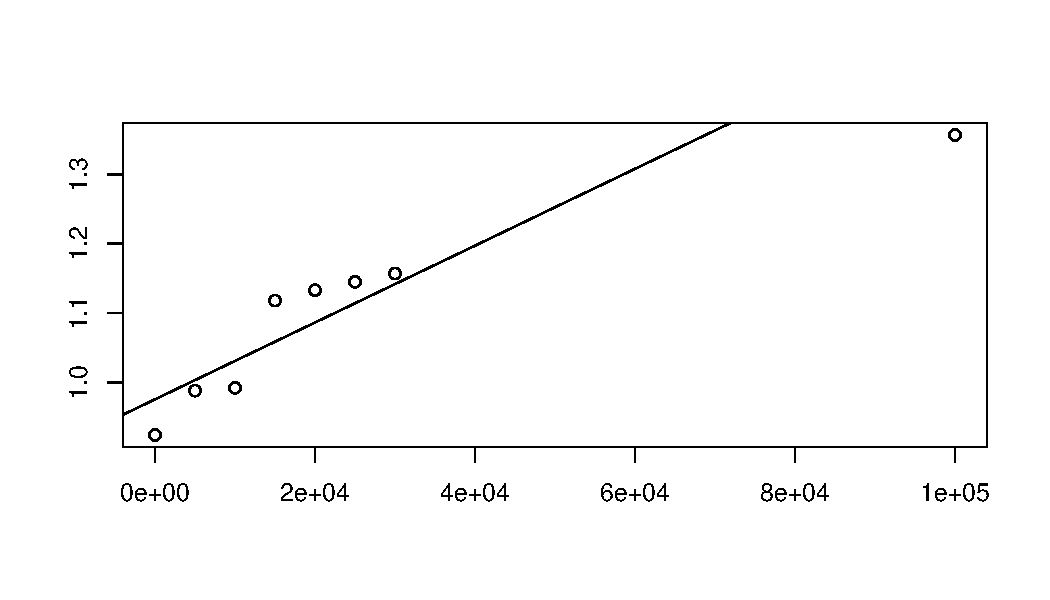
\includegraphics[width=\maxwidth]{figure/unnamed-chunk-2} 
\begin{kframe}\begin{alltt}
chemist_RBD_anova
\end{alltt}
\begin{verbatim}
## $`Analysis of variance`
##            df type III SS mean square F value    p>F
## treatments  3       12.95       4.317  2.3761 0.1211
## blocks      4      157.00      39.250 21.6055 <0.001
## Residuals  12       21.80       1.817       -      -
## 
## $`Adjusted means`
##   treatment adjusted.mean standard.error tukey snk duncan  t scott_knott
## 1        C4          72.6         0.6028     a   a      a  a           a
## 2        C3          72.4         0.6028     a   a     ab ab           a
## 3        C2          71.4         0.6028     a   a     ab ab           a
## 4        C1          70.6         0.6028     a   a      b  b           a
## 
## $`Multiple comparison test`
##      pair contrast p(tukey) p(snk) p(duncan)   p(t)
## 1 C4 - C3      0.2   0.9952 0.8185    0.8185 0.8185
## 2 C4 - C2      1.2   0.5183 0.3679    0.2050 0.1846
## 3 C4 - C1      2.0   0.1418 0.1418    0.0497 0.0370
## 4 C3 - C2      1.0   0.6540 0.2635    0.2635 0.2635
## 5 C3 - C1      1.8   0.2043 0.1291    0.0668 0.0564
## 6 C2 - C1      0.8   0.7853 0.3665    0.3665 0.3665
## 
## $`Residual analysis`
##                               values
## p.value Shapiro-Wilk test     0.0405
## p.value Bartlett test         0.7648
## coefficient of variation (%)  1.8800
## first value most discrepant  10.0000
## second value most discrepant 13.0000
## third value most discrepant  17.0000
\end{verbatim}
\begin{alltt}

\end{alltt}
\end{kframe}
\end{knitrout}



From the R code values, the F-value for the treatment is 2.38 with a corresponding p-value of 0.1211. So, null hypothesis can not be rejected. No significnt difference is visible among the chemical types at $\alpha = 0.05$ level. But the p-value for the blocks is very small. So, significant difference is visible for blocking. \\

\vspace{4 mm}

\section{ Exercise 4.4}

\begin{knitrout}
\definecolor{shadecolor}{rgb}{0.969, 0.969, 0.969}\color{fgcolor}\begin{kframe}
\begin{alltt}
\hlcomment{## RANDOMIZED BLOCK DESIGN}
\hlfunctioncall{setwd}(\hlstring{"C:/Users/Subasish/Dropbox/A Spring 2014/Dr Novelo/HW"})
bacteria_RBD <- \hlfunctioncall{read.csv}(\hlstring{"4.4.csv"})
\hlfunctioncall{head}(bacteria_RBD)
\end{alltt}
\begin{verbatim}
##   Solution Days Growth
## 1       S1   D1     13
## 2       S1   D2     22
## 3       S1   D3     18
## 4       S1   D4     39
## 5       S2   D1     16
## 6       S2   D2     24
\end{verbatim}
\begin{alltt}
toplot = \hlfunctioncall{matrix}(bacteria_RBD$Growth, byrow = TRUE, nrow = 3)
toplot
\end{alltt}
\begin{verbatim}
##      [,1] [,2] [,3] [,4]
## [1,]   13   22   18   39
## [2,]   16   24   17   44
## [3,]    5    4    1   22
\end{verbatim}
\begin{alltt}


modelRE = \hlfunctioncall{lmer}(Growth ~ (1 | Days) + Solution, data = bacteria_RBD)
\hlfunctioncall{summary}(modelRE)
\end{alltt}
\begin{verbatim}
## Linear mixed model fit by REML ['lmerMod']
## Formula: Growth ~ (1 | Days) + Solution 
##    Data: bacteria_RBD 
## 
## REML criterion at convergence: 60.37 
## 
## Random effects:
##  Groups   Name        Variance Std.Dev.
##  Days     (Intercept) 120.11   10.96   
##  Residual               8.64    2.94   
## Number of obs: 12, groups: Days, 4
## 
## Fixed effects:
##             Estimate Std. Error t value
## (Intercept)    23.00       5.67    4.05
## SolutionS2      2.25       2.08    1.08
## SolutionS3    -15.00       2.08   -7.22
## 
## Correlation of Fixed Effects:
##            (Intr) SltnS2
## SolutionS2 -0.183       
## SolutionS3 -0.183  0.500
\end{verbatim}
\begin{alltt}
\hlfunctioncall{anova}(modelRE, ddf = \hlstring{"lmer4"})
\end{alltt}
\begin{verbatim}
## Analysis of Variance Table
##          Df Sum Sq Mean Sq F value
## Solution  2    703     352    40.7
\end{verbatim}
\begin{alltt}

\hlcomment{##### ALTERNATIVE METHOD BY USING LIBRARY 'easyanova'}
bacteria_RBD_anova <- \hlfunctioncall{ea1}(bacteria_RBD, design = 2)
\end{alltt}
\end{kframe}
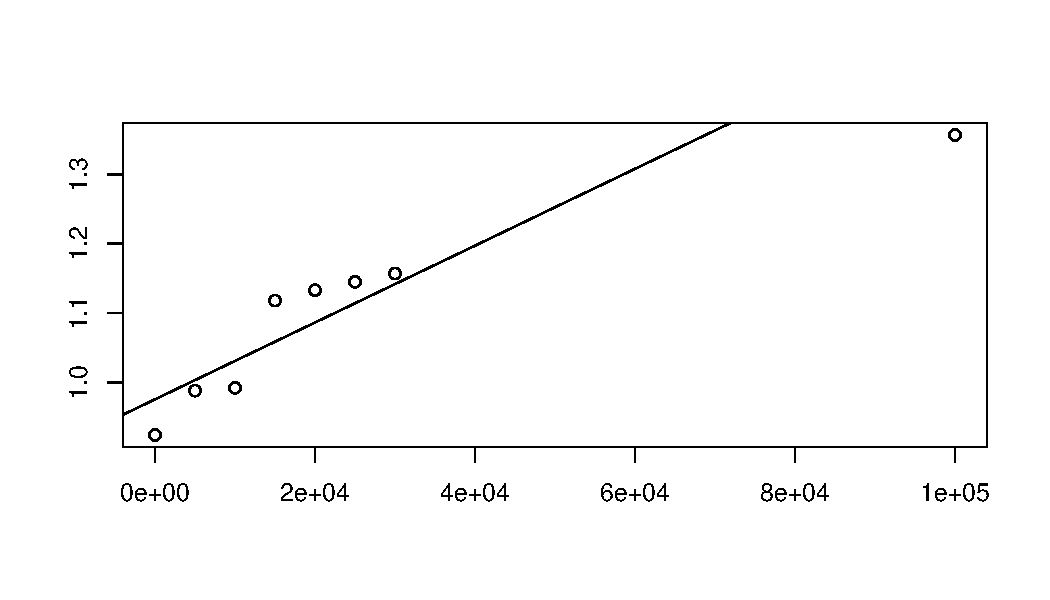
\includegraphics[width=\maxwidth]{figure/unnamed-chunk-3} 
\begin{kframe}\begin{alltt}
bacteria_RBD_anova
\end{alltt}
\begin{verbatim}
## $`Analysis of variance`
##            df type III SS mean square F value    p>F
## treatments  2      703.50     351.750  40.717 <0.001
## blocks      3     1106.92     368.972 42.7106 <0.001
## Residuals   6       51.83       8.639       -      -
## 
## $`Adjusted means`
##   treatment adjusted.mean standard.error tukey snk duncan t scott_knott
## 1        S2         25.25           1.47     a   a      a a           a
## 2        S1         23.00           1.47     a   a      a a           a
## 3        S3          8.00           1.47     b   b      b b           b
## 
## $`Multiple comparison test`
##      pair contrast p(tukey) p(snk) p(duncan)   p(t)
## 1 S2 - S1     2.25   0.5578 0.3206    0.3206 0.3206
## 2 S2 - S3    17.25   0.0004 0.0004    0.0002 0.0002
## 3 S1 - S3    15.00   0.0009 0.0004    0.0004 0.0004
## 
## $`Residual analysis`
##                               values
## p.value Shapiro-Wilk test     0.4027
## p.value Bartlett test         0.8803
## coefficient of variation (%) 15.6800
## first value most discrepant   9.0000
## second value most discrepant  1.0000
## third value most discrepant   8.0000
\end{verbatim}
\begin{alltt}

\end{alltt}
\end{kframe}
\end{knitrout}


From the R code values, the F-value for the treatment is 40.72 with a corresponding very small p-value. So, null hypothesis can be rejected. So, a clear difference is visible between the means of the three solutions. The blocking also shows some effect with F-value of 42.71 with lower p-value. The multiple comparison test indicates that solution 3 is significantly different than the other two solutions.\\

\vspace{4 mm}

\section{ Exercise 4.11}

(a)

\begin{knitrout}
\definecolor{shadecolor}{rgb}{0.969, 0.969, 0.969}\color{fgcolor}\begin{kframe}
\begin{alltt}
\hlcomment{## RANDOMIZED BLOCK DESIGN}
\hlfunctioncall{setwd}(\hlstring{"C:/Users/Subasish/Dropbox/A Spring 2014/Dr Novelo/HW"})
alg_RBD <- \hlfunctioncall{read.csv}(\hlstring{"4.11.csv"})
\hlfunctioncall{head}(alg_RBD)
\end{alltt}
\begin{verbatim}
##   Project Algorith Cost.Error
## 1      P1      SLM       1244
## 2      P2      SLM         21
## 3      P3      SLM         82
## 4      P4      SLM       2221
## 5      P5      SLM        905
## 6      P6      SLM        839
\end{verbatim}
\begin{alltt}
toplot = \hlfunctioncall{matrix}(alg_RBD$Cost.Error, byrow = TRUE, nrow = 6)
toplot
\end{alltt}
\begin{verbatim}
##      [,1] [,2] [,3] [,4] [,5] [,6]
## [1,] 1244   21   82 2221  905  839
## [2,]  281  129  396 1306  336  910
## [3,]  220   84  458  543  300  794
## [4,]  225   83  425  552  291  826
## [5,]   19   11  -34  121   15  103
## [6,]  -20   35  -53  170  104  199
\end{verbatim}
\begin{alltt}

modelRE = \hlfunctioncall{lmer}(Cost.Error ~ (1 | Project) + Algorith, data = alg_RBD)
\hlfunctioncall{summary}(modelRE)
\end{alltt}
\begin{verbatim}
## Linear mixed model fit by REML ['lmerMod']
## Formula: Cost.Error ~ (1 | Project) + Algorith 
##    Data: alg_RBD 
## 
## REML criterion at convergence: 451.5 
## 
## Random effects:
##  Groups   Name        Variance Std.Dev.
##  Project  (Intercept)  57714   240     
##  Residual             111183   333     
## Number of obs: 36, groups: Project, 6
## 
## Fixed effects:
##                         Estimate Std. Error t value
## (Intercept)                  560        168    3.34
## AlgorithCOCOMO-C            -159        192   -0.83
## AlgorithCOCOMO-R            -160        192   -0.83
## AlgorithESTIMALS            -487        192   -2.53
## AlgorithFUNCTION POINTS     -520        192   -2.70
## AlgorithSLM                  326        192    1.69
## 
## Correlation of Fixed Effects:
##             (Intr) ACOCOMO-C ACOCOMO-R AESTIM AFUNCP
## AlgCOCOMO-C -0.574                                  
## AlgCOCOMO-R -0.574  0.500                           
## AlgESTIMALS -0.574  0.500     0.500                 
## AFUNCTIONPO -0.574  0.500     0.500     0.500       
## AlgorithSLM -0.574  0.500     0.500     0.500  0.500
\end{verbatim}
\begin{alltt}
\hlfunctioncall{anova}(modelRE, ddf = \hlstring{"lmer4"})
\end{alltt}
\begin{verbatim}
## Analysis of Variance Table
##          Df  Sum Sq Mean Sq F value
## Algorith  5 2989130  597826    5.38
\end{verbatim}
\begin{alltt}

p_value <- 1 - \hlfunctioncall{pf}(5.38, 5, 25)
p_value
\end{alltt}
\begin{verbatim}
## [1] 0.001714
\end{verbatim}
\end{kframe}
\end{knitrout}


(b)

\begin{knitrout}
\definecolor{shadecolor}{rgb}{0.969, 0.969, 0.969}\color{fgcolor}\begin{kframe}
\begin{alltt}
\hlfunctioncall{plot}(modelRE)
\end{alltt}
\end{kframe}
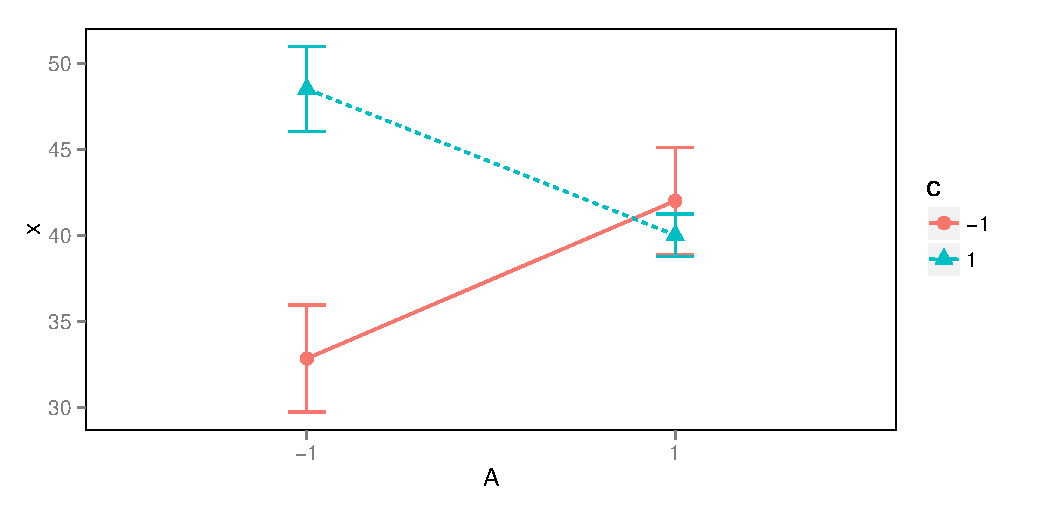
\includegraphics[width=\maxwidth]{figure/unnamed-chunk-5} 

\end{knitrout}


(c)

\begin{knitrout}
\definecolor{shadecolor}{rgb}{0.969, 0.969, 0.969}\color{fgcolor}\begin{kframe}
\begin{alltt}
modelRE
\end{alltt}
\begin{verbatim}
## Linear mixed model fit by REML ['lmerMod']
## Formula: Cost.Error ~ (1 | Project) + Algorith 
##    Data: alg_RBD 
## REML criterion at convergence: 451.5 
## Random effects:
##  Groups   Name        Std.Dev.
##  Project  (Intercept) 240     
##  Residual             333     
## Number of obs: 36, groups: Project, 6
## Fixed Effects:
##             (Intercept)         AlgorithCOCOMO-C         AlgorithCOCOMO-R  
##                     560                     -159                     -160  
##        AlgorithESTIMALS  AlgorithFUNCTION POINTS              AlgorithSLM  
##                    -487                     -520                      326
\end{verbatim}
\end{kframe}
\end{knitrout}


I will recommend Algorithm-SLIM for use in practice because it has only the possitive effect.


\vspace{4 mm}

\section{ Exercise 4.22}

\begin{knitrout}
\definecolor{shadecolor}{rgb}{0.969, 0.969, 0.969}\color{fgcolor}\begin{kframe}
\begin{alltt}
\hlcomment{### LATIN SQUARE DESIGN}
\hlfunctioncall{setwd}(\hlstring{"C:/Users/Subasish/Dropbox/A Spring 2014/Dr Novelo/HW"})
ingredient_LS <- \hlfunctioncall{read.csv}(\hlstring{"4.22.csv"})
\hlfunctioncall{head}(ingredient_LS)
\end{alltt}
\begin{verbatim}
##   Batch Day Catalyst Time
## 1    B1  D1        A    8
## 2    B2  D1        C   11
## 3    B3  D1        B    4
## 4    B4  D1        D    6
## 5    B5  D1        E    4
## 6    B1  D2        B    7
\end{verbatim}
\begin{alltt}

ingredient.lm <- \hlfunctioncall{lm}(Time ~ Day + Batch + Catalyst, ingredient_LS)
\hlfunctioncall{anova}(ingredient.lm)
\end{alltt}
\begin{verbatim}
## Analysis of Variance Table
## 
## Response: Time
##           Df Sum Sq Mean Sq F value  Pr(>F)    
## Day        4   12.2     3.1    0.98 0.45501    
## Batch      4   15.4     3.9    1.23 0.34762    
## Catalyst   4  141.4    35.4   11.31 0.00049 ***
## Residuals 12   37.5     3.1                    
## ---
## Signif. codes:  0 '***' 0.001 '**' 0.01 '*' 0.05 '.' 0.1 ' ' 1
\end{verbatim}
\begin{alltt}

ingredient.aov = \hlfunctioncall{aov}(Time ~ Day + Batch + Catalyst, ingredient_LS)
\hlfunctioncall{anova}(ingredient.aov)
\end{alltt}
\begin{verbatim}
## Analysis of Variance Table
## 
## Response: Time
##           Df Sum Sq Mean Sq F value  Pr(>F)    
## Day        4   12.2     3.1    0.98 0.45501    
## Batch      4   15.4     3.9    1.23 0.34762    
## Catalyst   4  141.4    35.4   11.31 0.00049 ***
## Residuals 12   37.5     3.1                    
## ---
## Signif. codes:  0 '***' 0.001 '**' 0.01 '*' 0.05 '.' 0.1 ' ' 1
\end{verbatim}
\begin{alltt}
\hlfunctioncall{par}(mfrow = \hlfunctioncall{c}(2, 2))
\hlfunctioncall{plot}(ingredient.aov)
\end{alltt}
\end{kframe}
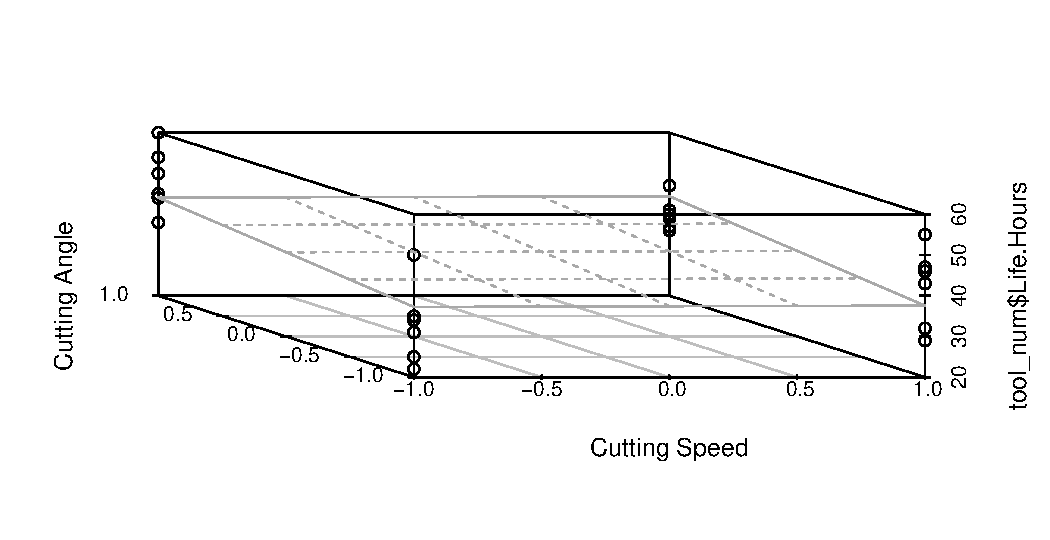
\includegraphics[width=\maxwidth]{figure/unnamed-chunk-7} 

\end{knitrout}



\begin{knitrout}
\definecolor{shadecolor}{rgb}{0.969, 0.969, 0.969}\color{fgcolor}\begin{kframe}
\begin{alltt}
\hlcomment{##### ALTERNATIVE METHOD BY USING LIBRARY 'easyanova'}
ingredient_LS1 <- ingredient_LS[\hlfunctioncall{c}(3, 1, 2, 4)]
\hlfunctioncall{head}(ingredient_LS1)
\end{alltt}
\begin{verbatim}
##   Catalyst Batch Day Time
## 1        A    B1  D1    8
## 2        C    B2  D1   11
## 3        B    B3  D1    4
## 4        D    B4  D1    6
## 5        E    B5  D1    4
## 6        B    B1  D2    7
\end{verbatim}
\begin{alltt}
alg_RBD_anova <- \hlfunctioncall{ea1}(ingredient_LS1, design = 3)
\end{alltt}
\end{kframe}
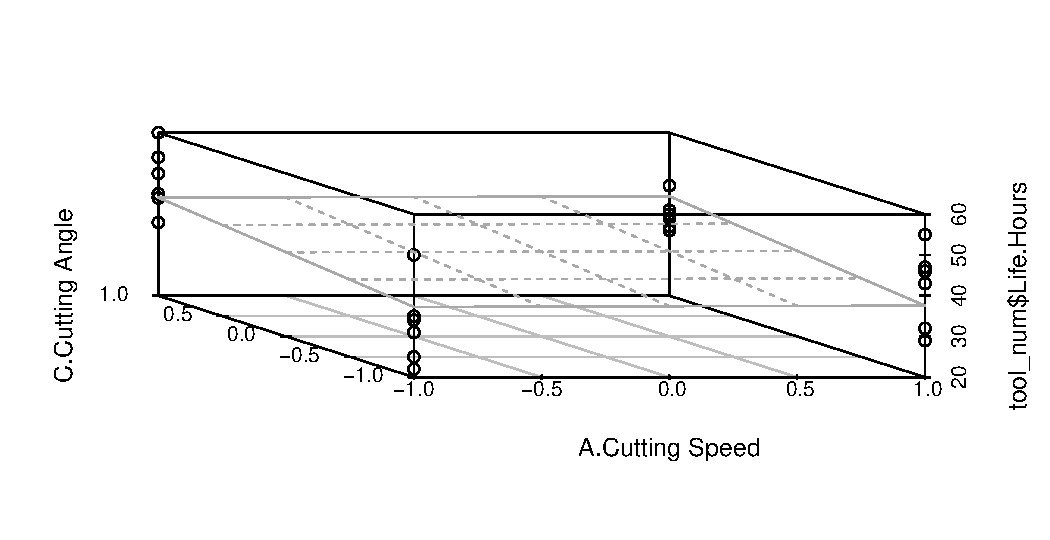
\includegraphics[width=\maxwidth]{figure/unnamed-chunk-8} 
\begin{kframe}\begin{alltt}
alg_RBD_anova
\end{alltt}
\begin{verbatim}
## $`Analysis of variance`
##            df type III SS mean square F value    p>F
## treatments  4      141.44      35.360 11.3092 <0.001
## rows        4       15.44       3.860  1.2345 0.3476
## columns     4       12.24       3.060  0.9787  0.455
## Residuals  12       37.52       3.127       -      -
## 
## $`Adjusted means`
##   treatment adjusted.mean standard.error tukey snk duncan t scott_knott
## 1         C           8.8         0.7908     a   a      a a           a
## 2         A           8.4         0.7908     a   a      a a           a
## 3         B           5.6         0.7908    ab   b      b b           b
## 4         D           3.4         0.7908     b   b      b b           b
## 5         E           3.2         0.7908     b   b      b b           b
## 
## $`Multiple comparison test`
##     pair contrast p(tukey) p(snk) p(duncan)   p(t)
## 1  C - A      0.4   0.9960 0.7268    0.7268 0.7268
## 2  C - B      3.2   0.0864 0.0355    0.0179 0.0143
## 3  C - D      5.4   0.0031 0.0020    0.0007 0.0004
## 4  C - E      5.6   0.0023 0.0023    0.0006 0.0003
## 5  A - B      2.8   0.1540 0.0277    0.0277 0.0277
## 6  A - D      5.0   0.0056 0.0020    0.0010 0.0008
## 7  A - E      5.2   0.0041 0.0027    0.0009 0.0006
## 8  B - D      2.2   0.3366 0.0727    0.0727 0.0727
## 9  B - E      2.4   0.2632 0.1220    0.0630 0.0530
## 10 D - E      0.2   0.9997 0.8611    0.8611 0.8611
## 
## $`Residual analysis`
##                               values
## p.value Shapiro-Wilk test     0.5476
## p.value Bartlett test         0.8170
## coefficient of variation (%) 30.0700
## first value most discrepant   6.0000
## second value most discrepant  3.0000
## third value most discrepant  14.0000
\end{verbatim}
\end{kframe}
\end{knitrout}


From the R code values, the F-value for the catalyst is 11.31 with a corresponding small p-value. So, null hypothesis can be rejected. So, the difference between the effect of five different ingredients  on the reaction time of a chemical process is somewhat significant. But for day and batches, the p-values are higher in values which indicate that they have no effect on the experiment. \\


\vspace{4 mm}

\section{ Exercise 4.24}

\begin{knitrout}
\definecolor{shadecolor}{rgb}{0.969, 0.969, 0.969}\color{fgcolor}\begin{kframe}
\begin{alltt}
\hlfunctioncall{setwd}(\hlstring{"C:/Users/Subasish/Dropbox/A Spring 2014/Dr Novelo/HW"})
bacteria_RBD <- \hlfunctioncall{read.csv}(\hlstring{"4.4.csv"})
\hlfunctioncall{head}(bacteria_RBD)
\end{alltt}
\begin{verbatim}
##   Solution Days Growth
## 1       S1   D1     13
## 2       S1   D2     22
## 3       S1   D3     18
## 4       S1   D4     39
## 5       S2   D1     16
## 6       S2   D2     24
\end{verbatim}
\begin{alltt}

modelRE = \hlfunctioncall{lmer}(Growth ~ (1 | Solution) + Days, data = bacteria_RBD)
\hlfunctioncall{summary}(modelRE)
\end{alltt}
\begin{verbatim}
## Linear mixed model fit by REML ['lmerMod']
## Formula: Growth ~ (1 | Solution) + Days 
##    Data: bacteria_RBD 
## 
## REML criterion at convergence: 51.76 
## 
## Random effects:
##  Groups   Name        Variance Std.Dev.
##  Solution (Intercept) 85.78    9.26    
##  Residual              8.64    2.94    
## Number of obs: 12, groups: Solution, 3
## 
## Fixed effects:
##             Estimate Std. Error t value
## (Intercept)   11.333      5.610    2.02
## DaysD2         5.333      2.400    2.22
## DaysD3         0.667      2.400    0.28
## DaysD4        23.667      2.400    9.86
## 
## Correlation of Fixed Effects:
##        (Intr) DaysD2 DaysD3
## DaysD2 -0.214              
## DaysD3 -0.214  0.500       
## DaysD4 -0.214  0.500  0.500
\end{verbatim}
\begin{alltt}
\hlfunctioncall{anova}(modelRE, ddf = \hlstring{"lmer4"})
\end{alltt}
\begin{verbatim}
## Analysis of Variance Table
##      Df Sum Sq Mean Sq F value
## Days  3   1107     369    42.7
\end{verbatim}
\begin{alltt}


\hlcomment{##### ALTERNATIVE METHOD BY USING LIBRARY 'easyanova'}
bacteria_RBD1 <- bacteria_RBD[\hlfunctioncall{c}(2, 1, 3)]
\hlfunctioncall{head}(bacteria_RBD1)
\end{alltt}
\begin{verbatim}
##   Days Solution Growth
## 1   D1       S1     13
## 2   D2       S1     22
## 3   D3       S1     18
## 4   D4       S1     39
## 5   D1       S2     16
## 6   D2       S2     24
\end{verbatim}
\begin{alltt}
bacteria_RBD_anova <- \hlfunctioncall{ea1}(bacteria_RBD1, design = 2)
\end{alltt}
\end{kframe}
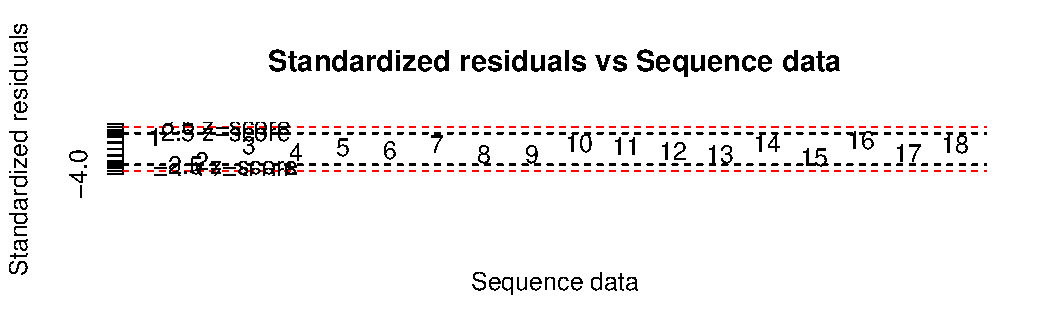
\includegraphics[width=\maxwidth]{figure/unnamed-chunk-9} 
\begin{kframe}\begin{alltt}
bacteria_RBD_anova
\end{alltt}
\begin{verbatim}
## $`Analysis of variance`
##            df type III SS mean square F value    p>F
## treatments  3     1106.92     368.972 42.7106 <0.001
## blocks      2      703.50     351.750  40.717 <0.001
## Residuals   6       51.83       8.639       -      -
## 
## $`Adjusted means`
##   treatment adjusted.mean standard.error tukey snk duncan t scott_knott
## 1        D4         35.00          1.697     a   a      a a           a
## 2        D2         16.67          1.697     b   b      b b           b
## 3        D3         12.00          1.697     b   b      b b           b
## 4        D1         11.33          1.697     b   b      b b           b
## 
## $`Multiple comparison test`
##      pair contrast p(tukey) p(snk) p(duncan)   p(t)
## 1 D4 - D2  18.3333   0.0011 0.0003    0.0003 0.0003
## 2 D4 - D3  23.0000   0.0003 0.0002    0.0001 0.0001
## 3 D4 - D1  23.6667   0.0003 0.0003    0.0001 0.0001
## 4 D2 - D3   4.6667   0.3038 0.0998    0.0998 0.0998
## 5 D2 - D1   5.3334   0.2193 0.1455    0.0756 0.0680
## 6 D3 - D1   0.6667   0.9917 0.7905    0.7905 0.7905
## 
## $`Residual analysis`
##                               values
## p.value Shapiro-Wilk test     0.4027
## p.value Bartlett test         0.8369
## coefficient of variation (%) 15.6800
## first value most discrepant   9.0000
## second value most discrepant  1.0000
## third value most discrepant   8.0000
\end{verbatim}
\end{kframe}
\end{knitrout}


From the R output, the F-value for the treatment is 42.71 with a corresponding small p-value. So, null hypothesis can be rejected. So, treatment has some effect. The blocks also generate F-value of 40.72 with lower p-value. So, blocking also has some effect.


\vspace{4 mm}

\section{ Exercise 4.35}

\begin{knitrout}
\definecolor{shadecolor}{rgb}{0.969, 0.969, 0.969}\color{fgcolor}\begin{kframe}
\begin{alltt}
\hlcomment{### Graeco-Latin Square Design}
\hlfunctioncall{setwd}(\hlstring{"C:/Users/Subasish/Dropbox/A Spring 2014/Dr Novelo/HW"})
chemical_GLS <- \hlfunctioncall{read.csv}(\hlstring{"4.35.csv"})
\hlfunctioncall{head}(chemical_GLS)
\end{alltt}
\begin{verbatim}
##   Batch Acid Time Catalyst Yield
## 1    B1   A1    A        a    26
## 2    B2   A1    B        c    18
## 3    B3   A1    C        e    20
## 4    B4   A1    D        b    15
## 5    B5   A1    E        d    10
## 6    B1   A2    B        b    16
\end{verbatim}
\begin{alltt}
chemical_GLS.aov = \hlfunctioncall{aov}(Yield ~ Acid + Batch + Catalyst + Time, chemical_GLS)
\hlfunctioncall{anova}(chemical_GLS.aov)
\end{alltt}
\begin{verbatim}
## Analysis of Variance Table
## 
## Response: Yield
##           Df Sum Sq Mean Sq F value  Pr(>F)    
## Acid       4     24     6.1    1.04 0.44254    
## Batch      4     10     2.5    0.43 0.78545    
## Catalyst   4     12     3.0    0.51 0.72890    
## Time       4    343    85.7   14.65 0.00094 ***
## Residuals  8     47     5.9                    
## ---
## Signif. codes:  0 '***' 0.001 '**' 0.01 '*' 0.05 '.' 0.1 ' ' 1
\end{verbatim}
\end{kframe}
\end{knitrout}


From the R output, the F-value of time is 14.65 with a corresponding p-value of 0.00094. So, null hypothesis can be rejected. We an say that time has some effect. But acid, batch and catalyst, the p-values are higher in value which indicate that they have no effect on the experiment. 


\vspace{4 mm}

\section{ Exercise 4.42}

\begin{knitrout}
\definecolor{shadecolor}{rgb}{0.969, 0.969, 0.969}\color{fgcolor}\begin{kframe}
\begin{alltt}
\hlcomment{### Balanced Incomplete Block Design (BIBD)}
\hlfunctioncall{setwd}(\hlstring{"C:/Users/Subasish/Dropbox/A Spring 2014/Dr Novelo/HW"})
hardwood_BIBD <- \hlfunctioncall{read.csv}(\hlstring{"4.42_1.csv"})
\hlfunctioncall{head}(hardwood_BIBD)
\end{alltt}
\begin{verbatim}
##   Concen Days Strength
## 1     C2   D1      114
## 2     C2   D2       NA
## 3     C2   D3       NA
## 4     C2   D4       NA
## 5     C2   D5      120
## 6     C2   D6       NA
\end{verbatim}
\begin{alltt}
toplot = \hlfunctioncall{matrix}(hardwood_BIBD$Strength, byrow = TRUE, nrow = 7)
toplot
\end{alltt}
\begin{verbatim}
##      [,1] [,2] [,3] [,4] [,5] [,6] [,7]
## [1,]  114   NA   NA   NA  120   NA  117
## [2,]  126  120   NA   NA   NA  119   NA
## [3,]   NA  137  114   NA   NA   NA  134
## [4,]  141   NA  129  149   NA   NA   NA
## [5,]   NA  145   NA  150  143   NA   NA
## [6,]   NA   NA  120   NA  118  123   NA
## [7,]   NA   NA   NA  136   NA  130  127
\end{verbatim}
\begin{alltt}

ingredient.lm <- \hlfunctioncall{lm}(Strength ~ Concen + Days, hardwood_BIBD)
\hlfunctioncall{anova}(ingredient.lm)
\end{alltt}
\begin{verbatim}
## Analysis of Variance Table
## 
## Response: Strength
##           Df Sum Sq Mean Sq F value  Pr(>F)    
## Concen     6   2040     340   13.52 0.00084 ***
## Days       6    442      74    2.93 0.08126 .  
## Residuals  8    201      25                    
## ---
## Signif. codes:  0 '***' 0.001 '**' 0.01 '*' 0.05 '.' 0.1 ' ' 1
\end{verbatim}
\end{kframe}
\end{knitrout}


From the R output, the F-value for the concentration is 13.52 with a corresponding p-value of 0.00084. So, null hypothesis can be rejected. We can say that concentration has some effect. For days, the p-value is slightly higher than 0.05 for days. It indicates that days have no effect on the experiment.


\vspace{4 mm}

\section{ Exercise 4.49}

\begin{knitrout}
\definecolor{shadecolor}{rgb}{0.969, 0.969, 0.969}\color{fgcolor}\begin{kframe}
\begin{alltt}
\hlcomment{### Verify that a BIBD with the parameters a =8, r =8, k =4, and b =16}
\hlcomment{### does not exist.}

a = 8
r = 8
k = 4
b = 16

lamda = r * (k - 1)/(a - 1)
lamda
\end{alltt}
\begin{verbatim}
## [1] 3.429
\end{verbatim}
\end{kframe}
\end{knitrout}


From the R output, it's found that the value of $\lambda$ is not an integer. So, a BIBD with these parameters cannot exist.

\end{document}
